\documentclass[%
	11pt,%
	a4paper,%
	twoside,
	%bibtotoc,%
	%liststotoc%
	]{scrreprt}


\usepackage[latin1,utf8]{inputenc}

%\usepackage[colorlinks=false]{hyperref}
				%colorlinks=true: Links von Referenzierungen in Farben, Nachteil: Bei Ausdruck auch in Farbe
				%colorlinks=false: Farbige Kaestchen und Ausdruck in Schwarz
\usepackage%
[colorlinks=true,
	citecolor=black,
	urlcolor=black,
	linkcolor=black]
{hyperref} %Alle Verlinkungen in schwarz.

%***hypersetup nur m\"oglich in Kombination mit hyperref!
\hypersetup{
	pdfauthor={Michael Ebner},
	pdftitle={RCCPP Coursework 01},
	%pdfkeywords={Reservoir Theory, Windkessel Model, Peripheral Arteries, Brachial Artery, Carotid Artery},
	%pdfsubject={Diploma Thesis} %Diplomarbeit, Seminararbeit etc
	%pdfcreationdate=20131204180532, 	%Ausgabe: Wednesday 04 December 2013 18:05:32
	%pdfmoddate=20131005 							%Ausgabe: Saturday 05 October 2013 00:00:00
	%Creation und modified date wird sowieso automatisch ausgegeben.
}

%***hypcap nur m\"oglich in Kombination mit hyperref!
\usepackage[all]{hypcap}  %Ohne dieser Zeile waere hyperref nur auf Caption unter Abbildung. Mit: ganze Abb. sichtbar

%***\texorpdfstring{''TEX text''}{''Bookmark Text''} %Interessant wenn Mathematische Formeln in \"Uberschriften
%***zB: \subsection{\texorpdfstring{$(h-h/2)$-Fehlersch\"atzer $\eta_\ell$ bzw. $\eta_\ell^*$}{(h-h/2)-Fehlersch\"atzer}}
%\newcommand{\texorpdfstring}[2]{#1} %Wenn Dokument ohne Hyperref erw\"unscht, dann wird Befehl \"uberschrieben --> keine Fehlermeldung

% Anpassen der Schriften des KOMA-Skripts:
%-----------------------------------------------------------------------------------------------------------------------
%Package noetig um gleiches font wie fuer ``article`` zu erhalten.
% \setkomafont{disposition}{\normalfont\bfseries}

% Aendert alle Gliederungsueberschriften (\part bis \subparagraph und \minisec) sowie Überschrift der Zusammenfassung
% Math-Umgebung wird in Ueberschrift fett angezeigt
\setkomafont{disposition}{\rmfamily\bfseries\boldmath}
 
% Aendert das Label (also den optionalen Eintrag einer \item-Anweisung) einer description-Umgebung 
%\setkomafont{descriptionlabel}{\rmfamily\bfseries\boldmath}   
%-----------------------------------------------------------------------------------------------------------------------
\usepackage[noadjust]{cite} %normal liefert \cite{} ein automatisches Leerzeichen vor Referenz; noadjust verhindert dies. Bsp: (\cite{test}) =( [2]) --> ([2])
\usepackage[ngerman,english]{babel}
\usepackage[T1]{fontenc}	%Damit wird zB auch \textsc{Matlab} in Kapitaelchen in Ueberschriften angezeigt
				%unbedingt "cm-super" installieren! sonst Schrift gerastert(pixelig) (alternative lmodern-package)
				%\usepackage{lmodern}		%mit [T1]{fontenc} Schrift "`pixelig"' (gerastert) -> lmodern verhindert dies.
\usepackage{ifthen,amsmath,amssymb,latexsym}
\usepackage{fancyhdr}
\usepackage{psfrag}
\usepackage{graphicx}
\usepackage[format=plain,justification=centering]{caption}
\usepackage{subfig}
% \captionsetup[subfloat]{captionskip=10pt}
\usepackage{mdframed}
% \usepackage{pgfplots}

\usepackage{listings}

\definecolor{mygreen}{rgb}{0,0.6,0}
\definecolor{mygray}{rgb}{0.5,0.5,0.5}
\definecolor{mymauve}{rgb}{0.58,0,0.82}
\definecolor{mybackgroundgray}{rgb}{0.9,0.9,0.9}
\definecolor{gray}{rgb}{0.75,0.75,0.75}
\definecolor{lightgray}{rgb}{0.95,0.95,0.95}

\lstdefinestyle{myCppStyle}{ %
	backgroundcolor=\color{mybackgroundgray},   % choose the background color; you must add \usepackage{color} or \usepackage{xcolor}
	basicstyle=\ttfamily\footnotesize,        % the size of the fonts that are used for the code
%	breakatwhitespace=false,         % sets if automatic breaks should only happen at whitespace
%	breaklines=true,                 % sets automatic line breaking
%	captionpos=b,                    % sets the caption-position to bottom
	commentstyle=\color{mygreen},    % comment style
%	deletekeywords={...},            % if you want to delete keywords from the given language
%	escapeinside={\%*}{*)},          % if you want to add LaTeX within your code
	extendedchars=true,              % lets you use non-ASCII characters; for 8-bits encodings only, does not work with UTF-8
%	frame=single,                    % adds a frame around the code
	keepspaces=true,                 % keeps spaces in text, useful for keeping indentation of code (possibly needs columns=flexible)
	keywordstyle=\color{blue},       % keyword style
	language=C++,                 % the language of the code
	morekeywords={pragma,omp,parallel,ifdef,endif},            % if you want to add more keywords to the set
	numbers=left,                    % where to put the line-numbers; possible values are (none, left, right)
%	numbersep=5pt,                   % how far the line-numbers are from the code
	numberstyle=\tiny\color{gray}, % the style that is used for the line-numbers
	rulecolor=\color{black},         % if not set, the frame-color may be changed on line-breaks within not-black text (e.g. comments (green here))
	showspaces=false,                % show spaces everywhere adding particular underscores; it overrides 'showstringspaces'
	showstringspaces=false,          % underline spaces within strings only
	showtabs=false,                  % show tabs within strings adding particular underscores
	stepnumber=1,                    % the step between two line-numbers. If it's 1, each line will be numbered
	stringstyle=\color{mymauve},     % string literal style
	tabsize=4,                       % sets default tabsize to 2 spaces
	%title=\lstname                   % show the filename of files included with \lstinputlisting; also try caption instead of title
}


\usepackage{cleveref}
\crefname{algorithm}{algorithm}{algorithms}

%***TikZ

\usepackage{fp,tikz}       %fixed point arithmetic for tex, tikz f\"ur Befehl foreach
% \usetikzlibrary{snakes}	%for underbraces
\usetikzlibrary{patterns,calc,intersections,arrows}

\newcommand*{\rechterWinkel}[3]{% #1 = point, #2 = start angle, #3 = radius
   \draw[shift={(#2:#3)}] (#1) arc[start angle=#2, delta angle=90, radius = #3];
   \fill[shift={(#2+45:#3/2)}] (#1) circle[radius=1.25\pgflinewidth];
}

\usepackage{enumitem}

\usepackage[
	separate-uncertainty=true,
	scientific-notation=false,
	%multi-part-units=single,
	list-units=repeat,
	per-mode = symbol
	]
	{siunitx}
%[ %
%	separate-uncertainity=true
%    ,uncertainity-separator={\pm}
        %mode = text,
%   ,multi-part-units = brackets
%	,decimalsymbol=comma
%]    

\sisetup{binary-units=true,separate-uncertainty}

% \usepackage{layout}
% \setlength{\marginparwidth}{0pt}

%\usepackage{pifont} %F\"ur q.e.d


%\setlength\parindent{0pt} %Festlegen des Absatzeinzuges

% %---F\"ur Symbolverzeichnis, Abk\"urzungsverz. und Glossaries:
% \usepackage[ngerman]{translator}
% \usepackage[
% 	nonumberlist, %keine Seitenzahlen anzeigen
% 	acronym,      %ein Abkuerzungsverzeichnis erstellen
% 	toc]          %Eintraege im Inhaltsverzeichnis
% 	%section]      %im Inhaltsverzeichnis auf section-Ebene erscheinen %nicht bei scrreprt
% 	{glossaries}

%\numberwithin{equation}{section} %koppelt Counter equation an chapter
%\numberwithin{figure}{section} %koppelt Counter figure an chapter


%---Tabellen (tabular) Formatierung:
%-Der Abstand zwischen den Zeilen einer Tabelle kann über folgenden Befehl angepasst werden:
%-\renewcommand{\arraystretch}{Faktor}
\renewcommand{\arraystretch}{1.2}
\usepackage{colortbl} %Paket notwending, dass arrayrulecolor ge\"andert werden kann
\arrayrulecolor[gray]{0.8}  %Linienfarbe der Tabelle
\usepackage{array}
\newcolumntype{L}[1]{>{\raggedright\let\newline\\\arraybackslash\hspace{0pt}}m{#1}}
\newcolumntype{C}[1]{>{\centering\let\newline\\\arraybackslash\hspace{0pt}}m{#1}}
\newcolumntype{R}[1]{>{\raggedleft\let\newline\\\arraybackslash\hspace{0pt}}m{#1}}

%---Formatierung bei zB enumerate Umgebung: Einfach \begin{enumerate}[(a)] oder ..[I] eingeben
%\usepackage{paralist}

\usepackage{multirow}
\def\R{\mathbb{R}}
\def\N{\mathbb{N}}

\def\x{\mathbf{x}}
\def\y{\mathbf{y}}
\def\n{\mathbf{n}}
\def\t{\mathbf{t}}
\def\v{\mathbf{v}}
\def\0{\mathbf{0}}

\def\p{\mathbf{p}}
\def\pp{\mathbf{p}^\prime}
\def\ppp{\mathbf{p}^{\prime\prime}}

\def\q{\mathbf{q}}
\def\qp{\mathbf{q}^\prime}
\def\qpp{\mathbf{q}^{\prime\prime}}

\def\qR{{\mathbf{q}_\text{\rm R}}}
\def\qT{{\mathbf{q}_\text{\rm T}}}
\def\mup{{\boldsymbol{\mu}_\text{\rm p}}}
\def\mux{{\boldsymbol{\mu}_\text{\rm x}}}

\def\DDelta{{\boldsymbol{\Delta}}}
\def\Sigmapx{{\boldsymbol{\Sigma}_\text{\rm px}}}


\def\AA{\mathbf{A}}
\def\HH{\mathbf{H}}
\def\II{\mathbf{I}}
\def\QQ{\mathbf{Q}}
\def\RR{\mathbf{R}}
\def\TT{\mathbf{T}}
\def\UU{\mathbf{U}}
\def\VV{\mathbf{V}}
\def\XX{\mathbf{X}}

\def\LLambda{\mathbf{\Lambda}}


\def\MyLineWidth{1pt}

\newcommand{\FRE}{{\text{\rm FRE}}}

\newcommand{\norm}[2][]{\ifthenelse{\equal{#1}{}}{\left\Vert #2 \right\Vert_{\ell^2}}{\left\Vert #2\right\Vert_{#1}}}

\DeclareMathOperator{\tr}{tr}
%%%%%%%%%%%%%%%%%%%%%%%%%%%%%%%%%%%%
% UMGEBUNG FUER CODE-DOKUMENTATION %
%%%%%%%%%%%%%%%%%%%%%%%%%%%%%%%%%%%%
\newenvironment{explain}{\begin{list}{\LARGE\color{gray}$\bullet$}{%
\setlength{\labelsep}{3mm}% davor 2.3mm
\setlength{\labelwidth}{1mm}% davor 3mm
\setlength{\leftmargin}{8mm}% davor 7mm
\setlength{\itemsep}{0mm}%
}}{\end{list}}


%Makro f\"ur aufeinander folgende Erh\"ohung der Lemma-/Satz-/Definitions- und Algorithmus-Counter
\newcommand{\updateCtr}[1]{
	\addtocounter{helper}{1}	%Master-Ctr inkrementieren
	
	\FPset\dummy{\thehelper}  %Da Befehl refstepcounter auch um eines erh\"oht, w\"urde ohne diese Zeilen
	\FPsub\dummy\thehelper{1} %erster Counter-Wert gleich 2 sein.
	\FPclip\dummy\dummy
	
	\setcounter{#1}{\dummy}
	\refstepcounter{#1}
}

%---Counter:
%%%%%%%%%%%%%%%%%%%%%%%%%%%%%%%%%%%%%%%%%%%%%%%%%%%%%%%%%%%%%%%%%%%%%%%%%%%%%%%%%%%%%%%%%%%%%%%%%%%%%%%%%%%%%%%%%%%%%%%%%%%%%
% \newcounter{const}
\newcounter{helper}[section] %sorgt f\"ur fortlaufende Nummerierung bei Satz/Lemma/Algorithmus/Definition
% \newcounter{satz}[section] %neuer counter; reset des counters bei neuer section
% \newcounter{lemma}[section]
\newcounter{algorithm}[section]
% \newcounter{definition}[section]

\numberwithin{equation}{section} %koppelt Counter equation an section
%\numberwithin{lstlisting}{section}

% \renewcommand{\theconst}{\arabic{const}}
% \renewcommand{\thesatz}{\arabic{section}.\arabic{satz}}           %Ausgabe bei Referenzierung
% \renewcommand{\thelemma}{\arabic{section}.\arabic{lemma}}
% \renewcommand{\thedefinition}{\arabic{section}.\arabic{definition}}
\renewcommand{\thealgorithm}{\arabic{section}.\arabic{algorithm}}
\renewcommand{\theequation}{\arabic{section}.\arabic{equation}}
% \renewcommand{\thesubfigure}{\,(\alph{subfigure})}

\renewcommand{\labelenumi}{(\arabic{enumi})}

\renewcommand\appendix{%\par 
	\numberwithin{lstlisting}{section} %Zaehler lstlisting im Anhang auf Null setzen -> Listing A.1 (ohne Listing 1 zu verlinken!)
	\renewcommand\thesection{A}% 
  \renewcommand\thesubsection{A.\arabic{subsection}}% 
  %\renewcommand\thefigure{\Alph{section}.\arabic{figure}}%
	\renewcommand\thelstlisting{A.\arabic{lstlisting}}%
}

%---Umgebungen:
%%%%%%%%%%%%%%%%%%%%%%%%%%%%%%%%%%%%%%%%%%%%%%%%%%%%%%%%%%%%%%%%%%%%%%%%%%%%%%%%%%%%%%%%%%%%%%%%%%%%%%%%%%%%%%%%%%%%%%%%%%%%%
% \renewenvironment{quote}% %Veraendern der Einz\"uge innerhalb der quote-Umgebung.
% {\begin{list}{}{% 
%   \setlength{\leftmargin}{0.5cm}%
%   \setlength{\rightmargin}{0.5cm}}%
%   \item[]\ignorespaces}%
% {\unskip\end{list}}

\newenvironment{satz}[1][]%
{%\begin{satz}

  \updateCtr{satz}%
  \medskip\noindent\begin{mdframed}[linewidth=\MyLineWidth]\noindent\textbf{\textit{Satz~\arabic{section}.\arabic{satz}%
  \ifthenelse{\equal{#1}{}}{}{~(#1).}}} \it
}
{%\end{satz}
  \end{mdframed}
  
  \medskip

}

\newenvironment{satzob}[1][]%Satz ohne Beweis
{%\begin{satzob}

  \updateCtr{satz}%
  \medskip\noindent\begin{mdframed}[linewidth=\MyLineWidth]\noindent\textbf{\textit{Satz~\arabic{section}.\arabic{satz}%
  \ifthenelse{\equal{#1}{}}{}{~(#1).}}} \it
}
{%\end{satzob}
	\hfill \squareShadow

	\end{mdframed}
	\bigskip

}

\newenvironment{beweis}[1][]%
{%\begin{beweis}
  \noindent\textsc{Beweis\ifthenelse{\equal{#1}{}}{:}{~von~{#1}:}}
}
{%end{beweis}
  \hfill \squareShadow
  \bigskip

}

\newenvironment{lemma}[1][]%
{%\begin{lemma}

  \updateCtr{lemma}%
  \bigskip\noindent\textbf{\textit{Lemma~\arabic{section}.\arabic{lemma}%
  \ifthenelse{\equal{#1}{}}{}{~(#1).}}} \it
}
{%\end{lemma}
  \hfill \squareShadow
  \bigskip

}
\newenvironment{lemmamb}[1][]%Satz MIT Beweis. NICHT KONSISTENT!?!?
{%\begin{lemmamb}

  \updateCtr{lemma}%
  \medskip\noindent\textbf{\textit{Lemma~\arabic{section}.\arabic{lemma}%
  \ifthenelse{\equal{#1}{}}{}{~(#1).}}} \it
}
{%\end{satzmb}

	\bigskip

}
\newenvironment{definition}[1][]%
{%\begin{definition}

  \updateCtr{definition}%
  \bigskip\noindent\textbf{\textit{Definition~\arabic{section}.\arabic{definition}%
  \ifthenelse{\equal{#1}{}}{}{~(#1).}}} \it
}
{%\end{definition}
  \bigskip

}

\newenvironment{algorithm}[1][]%
{%\begin{algorithm}
  \updateCtr{algorithm}%
	\medskip\noindent\begin{mdframed}[linewidth=\MyLineWidth,backgroundcolor=mybackgroundgray% %,innerleftmargin=12,innerrightmargin=12%
	]\noindent\textbf{\textit{Algorithm~\arabic{section}.\arabic{algorithm}%
  \ifthenelse{\equal{#1}{}}{}{~(#1).}}} \it
}
{%\end{algorithm}
	\end{mdframed}
	
  \bigskip

}

% \newenvironment{beispiel}[1][]
% {%\begin{beispiel}
%   \bigskip%
%   \noindent\refstepcounter{satz}\textbf{\textit{Beispiel~\arabic{section}.\arabic{satz}%
%   \ifthenelse{\equal{#1}{}}{}{~(#1).}}}% 
%   %\hangafter=1\hangindent=2em
% }
% {%\end{beispiel}
%   \bigskip
% }

%---Page Setup
%%%%%%%%%%%%%%%%%%%%%%%%%%%%%%%%%%%%%%%%%%%%%%%%%%%%%%%%%%%%%%%%%%%%%%%%%%%%%%%%%%%%%%%%%%%%%%%%%%%%%%%%%%%%%%%%%%%%%%%%

%---Define page:
\usepackage{geometry}
% % \geometry{hmargin=3cm, top=2cm, bottom=2cm, head=1cm, headsep=1cm, footskip=1.5cm, includeheadfoot,bindingoffset=1cm}
\geometry{
	a4paper,
	textwidth = 17cm, 
	top = 1.5cm, 
	bottom = 2cm, 
	head = 1cm, 
	headsep = 1cm, 
	footskip = 1.5cm, 
	includeheadfoot, 
	bindingoffset = 1.2cm
} %bindinoffset=1.2cm, dann mittig
% % includeheadfoot: Kopf-und Fusszeile in Seitenabmessungen miteinbezogen.

%---Kopf- und Fusszeile:
\pagestyle{fancy}
\renewcommand{\sectionmark}[1]{\markboth{\thesection.\ #1}{}}
\renewcommand{\subsectionmark}[1]{\markright{\thesubsection.\ #1}{}}
% \lhead{\leftmark}
% \chead{}
% \rhead{\rightmark}
% \lfoot{}
% \cfoot{\thepage}
% \rfoot{}

\fancyhead{}
\fancyhead[LE]{\slshape \leftmark} 	%bzw. LE,L0
\fancyhead[RO]{\slshape \rightmark} %bzw. RO
\fancyfoot[C]{\thepage}
%\fancyfoot[LO]{Michael Ebner}


% \usepackage{footnote}
%notwendig um mittels \begin{savenotes}..\end{savenotes} footnotes in table-Umgebung am Seitenende auszugeben.
%Besser am Ende laden, da es sonst zu Konflikten mit anderen Packages kommen kann.

%%%%%%%%%%%%%%%%%%%%%%%%%%%%%%%%%%%%%%%%%%%%%%%%%%%%%%%%%%%%%%%%%%%%%%%%%%%%%%%%%%%%%%%%%%%%%%%%%%%%%%%%%%%%%%%%%%%%%%%%%%%%%
%%% Dokumentbeginn
%%%%%%%%%%%%%%%%%%%%%%%%%%%%%%%%%%%%%%%%%%%%%%%%%%%%%%%%%%%%%%%%%%%%%%%%%%%%%%%%%%%%%%%%%%%%%%%%%%%%%%%%%%%%%%%%%%%%%%%%%%%%%
\begin{document}

%---Kopf- und Fusszeile:-----------------------------------------------------------------------------------------------------
\pagestyle{fancy}
%\renewcommand{\sectionmark}[1]{\markboth{\thesection.\ #1}{}}
%\renewcommand{\subsectionmark}[1]{\markright{\thesubsection.\ #1}{}}
\lhead{\leftmark}
\chead{}
\rhead{\rightmark}
\lfoot{}
\cfoot{\thepage}
\rfoot{}

%---Dokumentbeschriftungen:
\title{Parallel Implementation of the Game of Life}
\subject{MPHYG002: Research Computing with C++}
\author{Michael Ebner\\(Student Number: 15001660)}
%\publishers{Betreut durch Dipl.-Ing. Andreas K\"orner}


%---Title page(s)
%%%%%%%%%%%%%%%%%%%%%%%%%%%%%%%%%%%%%%%%%%%%%%%%%%%%%%%%%%%%%%%%%%%%%%%%%%%%%%%%%%%%%%%%%%%%%%%%%%%%%%%%%%%%%%%%%%%%%%%%

\pagenumbering{roman}
\maketitle           
\thispagestyle{empty} 
\cleardoublepage

\pagestyle{plain}     %keine Kopfzeile auf Inhaltsverzeichnisseite
\tableofcontents      
\cleardoublepage

\pagestyle{fancy}
\setcounter{page}{1}
\pagenumbering{arabic}

%---Eigentlicher Dokumentbeginn:---------------------------------------------------------------------------------------------
\chapter{Conways Game of Life}

Based on the lecture notes and \url{http://en.wikipedia.org/wiki/Conways_Game_of_Life}\footnote{Retrieved: April 25, October 2015} the concept of the game can be understood as a simulation of a population change over time. The rules read as follows:
\begin{itemize}
	\item The game is represented by an infinite two-dimensional grid of cells.
	\item Every cell can represent two possible states: dead or alive.
	\item The grid with its cells represent a population at a discrete point of time.
	\item The state of each cell in the consecutive time step depends on its 8 adjacent neighbours.
	\item The transition of the each cell's state are described by these rules (Summary is given in \cref{table:rules}):
	\begin{itemize}
		\item A live cell remains alive in case it is surrounded by either two or three living cells. Otherwise it dies which relates to the cases of under-population or overcrowding respectively.
		\item A dead cell with exactly three surrounding living cells becomes alive associated with the idea of reproduction.
	\end{itemize}
\end{itemize}

\begin{table}[h]\centering
	\begin{tabular}{c c | c c c c c c c c c} \hline\hline
		& & \multicolumn{9}{c}{\bf Number of neighbour cells alive} \\
		& & \bf 0 & \bf 1 & \bf 2 & \bf 3 & \bf 4 & \bf 5 & \bf 6 & \bf 7 & \bf 8 \\ \hline
		\multirow{2}{*}{\bf Current state} & \bf 0 & 0 & 0 & 0 & 1 & 0 & 0 & 0 & 0 & 0 \\
		& \bf 1 & 0 & 0 & 1 & 1 & 0 & 0 & 0 & 0 & 0 \\
		\hline\hline
	\end{tabular}
	\caption[Transition rules]{Transition rules: "0" indicates a dead and "1" a live cell}
	\label{table:rules}
\end{table}



\chapter{Implementation}


\section{Structure of project-folder}
The project can be downloaded from \url{https://github.com/renbem/RCCPP-coursework02}. The code is structured in several folders within the main directory:
\begin{itemize}
	\item \texttt{documentation:} Contains all documentation of the project including this report and the code documentation generated by doxygen\footnote{\url{www.doxygen.org}}.
	\item \texttt{include:} Contains all header files (\texttt{*.h})
	\item \texttt{matlab:} Contains the \textsc{Matlab}-files used for the random generation of initial boards (or grid according to the terminology used in chapter 1), the creation of the Game of Life video\footnote{Provided at \url{https://www.youtube.com/watch?v=AeIm2I_9n5g&feature=youtu.be}} and statistical evaluation of the results.
	\item \texttt{source:} Contains the code files (\texttt{*.cc} including \texttt{main.cc}).
	\item \texttt{test:} Contains all data and the source file \texttt{main\_UnitTests.cc} for the unit tests.
\end{itemize}

\section{Choice of design}
The implementation follows the design as illustrated in \cref{fig:OverviewOfImplementation} which translates the concept of a having a game consisting of boards which in turn consist of cells.

The classes are designed so that a new iteration is triggered by the member function \texttt{computeNextStep} of \texttt{Game}, cf. \cref{fig:computeNextStepCall}. I decided to connect the "rules of the game" with the board via the two methods \texttt{determineNeighbourCells} and \texttt{applyTransitionRules} since they constitute two separate logical units. However, one could argue that this might be better situated in the class \texttt{Game} since the rules can be considered as an intrinsic property of the game and the board could be of arbitrary shape\footnote{E.g. circular, hexagonal, $x$-dimensional, etc.}. Nevertheless, since Conway's Game of Life relies on well-balanced rules in order to have a "meaningful game" (i.e. no extinction or overcrowding of cells) the definition of a neighbour and the propagation rules depend strongly on the shape and therefore on the board.

\begin{figure}
	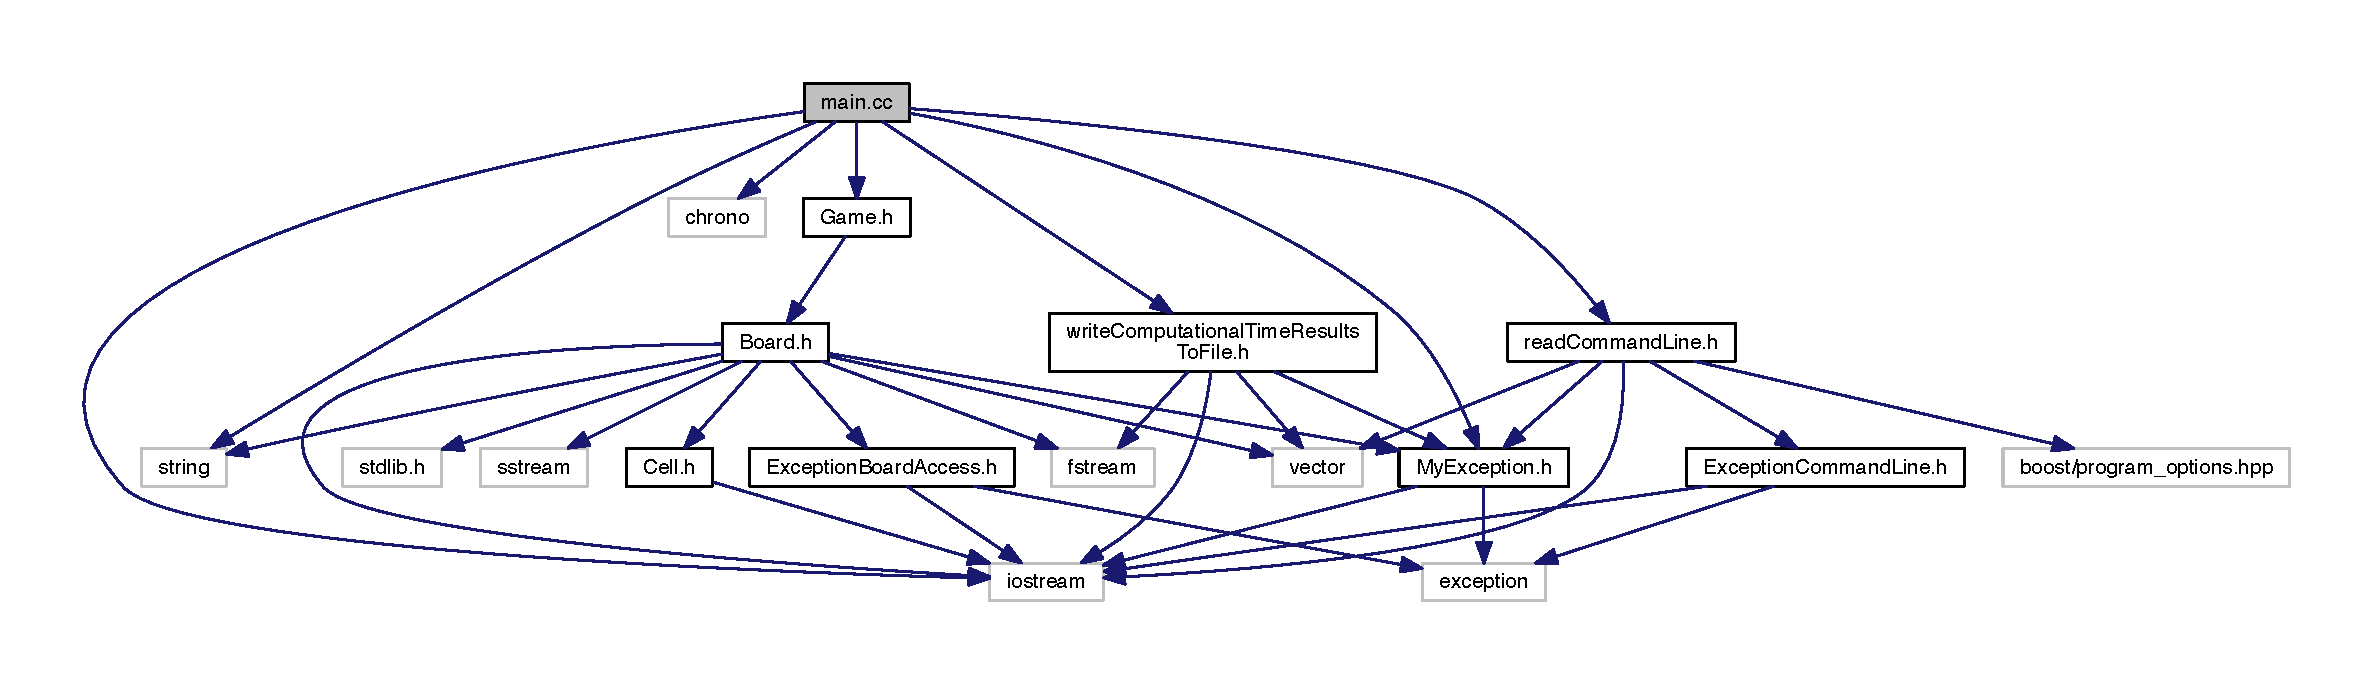
\includegraphics[width=\textwidth]{doxygen/latex/a00143.pdf}
	\caption{Overview of implementation}
	\label{fig:OverviewOfImplementation}
\end{figure}


\begin{figure}
	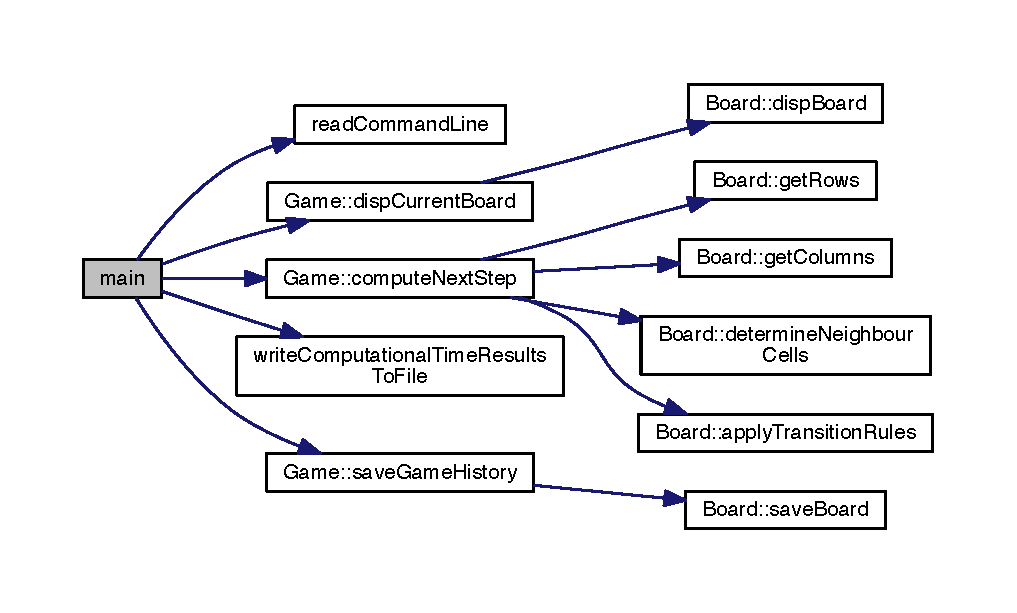
\includegraphics[width=\textwidth]{doxygen/latex/a00108_a3c04138a5bfe5d72780bb7e82a18e627_cgraph.pdf}
	\caption{Call graph of \texttt{main.cc}}
	\label{fig:computeNextStepCall}
\end{figure}

%It was aimed that a minimal amount of methods are defined as public to fulfil their purpose. The public methods of these three classes are illustrated in \cref{fig:MainClasses}.
%
%\begin{figure}\centering
%	\subfloat[\texttt{Game}]{\label{fig:Game}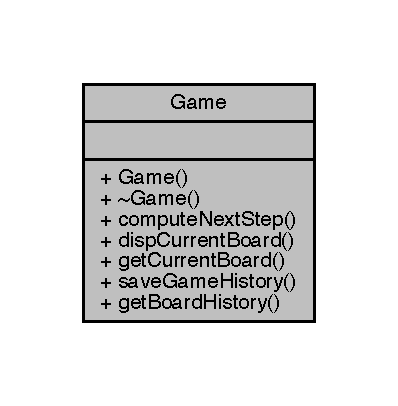
\includegraphics[width=0.33\textwidth]{doxygen/latex/a00165.pdf}}
%	\subfloat[\texttt{Board}]{\label{fig:Board}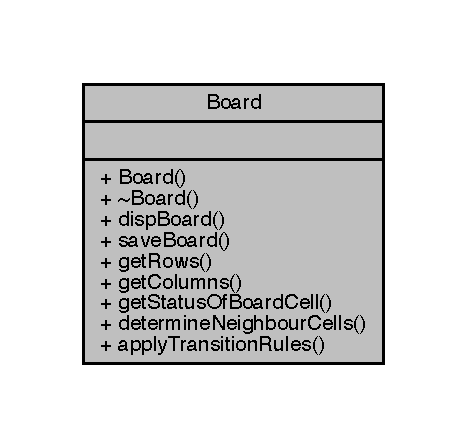
\includegraphics[width=0.33\textwidth]{doxygen/latex/a00155.pdf}}
%	\subfloat[\texttt{Cell}]{\label{fig:Cell}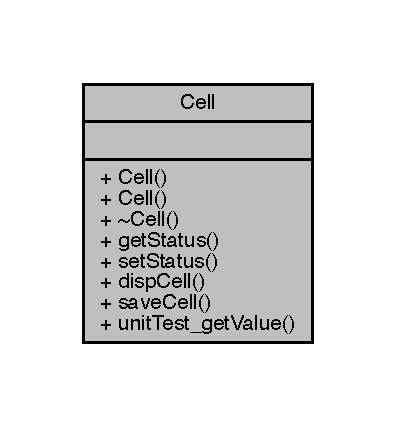
\includegraphics[width=0.33\textwidth]{doxygen/latex/a00157.pdf}}
%	\caption{Main classes of implementation and their public methods}
%	\label{fig:MainClasses}
%\end{figure}

\section{Parallelisation}
The code was parallelised via \textbf{OpenMP} within the method \texttt{computeNextStep}, cf. line 10 in \cref{Gamecc}. The line 9 and 11 was added since I could not compile it without any error messages on Mac (further information in \cref{sec:BuildRunTest}) but it works on Ubuntu. Therefore, the code runs on non-linux platforms only in the serial version.


\lstinputlisting
[style=myCppStyle,caption={Game::computeNextStep},label=Gamecc,belowskip=7mm,frame=lines,linerange={29-49}]
{../source/Game.cc}

\section{Unit tests}
Unit tests were written to test the following cases:
\begin{itemize}
	\item Check input file\footnote{It is only tested whether the input file exists. Many other cases could be tested in addition. E.g.: Format of file appropriate?, Number of columns always identical?, Minimum number of rows and columns alright? etc.}.
	\item Several tests to check malformed command lines.
	\item Several tests to check whether the correct neighbours are returned by \texttt{Board::neighbourCells}. (The "infinite board" was implemented by assuming periodic boundary conditions.)
	\item Check that attempted access to non-existing indices of board throws an exception.
	\item Test whether one step of Conway's Game of Life is computed correctly.
	\item Test whether the parallel computation via OpenMP returns the same board as the serial version.
	
\end{itemize}
The corresponding file \texttt{main\_UnitTests.cc} is located in \texttt{test/}.

\section{Build, run and test}\label{sec:BuildRunTest}
The \texttt{CMakeLists.txt} file in the parent directory was tested on two operating systems:

\begin{itemize}
	\item OS X 10.10.3 (Macbook Pro, 2.5 GHz Intel Core i7)
	\item Ubuntu 14.04 (Virtual machine via VirtualBox\footnote{\url{https://www.virtualbox.org/}} within OS X 10.10.3)
\end{itemize}

Unfortunately, I couldn't run OpenMP on Mac without any errors (comments are provided in the \texttt{CMakeLists.txt} file). Therefore, I used VirtualBox to build it on Ubuntu where everything went flawlessly. Consequently, I configured the CMake file (and added respective lines in \texttt{Game.cc}, e.g. lines 9 and 11 in \cref{Gamecc}) so that the code runs on Mac in serial and on Ubuntu with OpenMP. The results in \cref{sec:results} are based on the computation in Ubuntu.


\subsection{Build instructions}
In order to build the code run the following lines in the main directory:
\begin{quote}
	\texttt{mkdir build}\\
	\texttt{cd build}\\
	\texttt{cmake ..}\\
	\texttt{make}
\end{quote}
Two binary files will be generated:
\begin{itemize}
	\item \texttt{conwaysGameOfLife} located in \texttt{build/bin/}
	\item \texttt{conwaysGameOfLife\_UnitTests} located in \texttt{build/test/bin/}
\end{itemize}


\subsection{Running the programme}
For running the code several example data sets are provided in \texttt{build/test/exampleData/}.
A possible command of the programme within the \texttt{build}-folder reads
\begin{quote}
	\texttt{bin/conwaysGameOfLife -{}-i "test/exampleData/InitialBoardRandom\_10Times10.txt" -{}-o "GameHistory.txt" -{}-s 100}
\end{quote}
which uses the initial board defined in \texttt{InitialBoardRandom\_10Times10.txt} and performs 100 steps by applying the transition rules given in \cref{table:rules}. A concatenated history of all computed boards is then stored in \texttt{GameHistory.txt} and the information of the corresponding computational time per iteration is saved in \texttt{GameHistory\_ComputationalTime.txt}.

Alternatively any other file \texttt{InitialBoardRandom\_*.txt} in \texttt{test/exampleData} can be used as input file\footnote{A "on-screen-simulation" and its corresponding computational time can also be enabled by setting the respective flags \texttt{flagDisplayGame} and \texttt{flagDisplayComputationalTime} to \texttt{true} within \texttt{main.cc}.}.

\subsection{Run unit tests}
To run the unit tests, execute the command
\begin{quote}
	\texttt{./conwaysGameOfLife\_UnitTests}
\end{quote}
in \texttt{build/test/bin/}.


\section{Results}\label{sec:results}
In this section the results, obtained on Ubuntu, are shown and shall be discussed.

\subsection{Video}
An example board of dimension $200\times 400$ was computed and uploaded to \url{https://www.youtube.com/watch?v=AeIm2I_9n5g&feature=youtu.be}. Several phenomena can be observed such as gliders, oscillators and stationary patterns.

\subsection{Parallel vs. serial implementation}
In this comparison the Game of Life rules were applied to boards of dimensions
\begin{multicols}{2}
	\begin{enumerate}[label=(\roman*),leftmargin=2cm]
		\item $10\times10$ (100 Cells)
		\item $10\times20$ (200 Cells)
		\item $10\times50$ (500 Cells)
		\item $10\times100$ (\num{1000} Cells)
		\item $50\times100$ (\num{5000} Cells)
		\item $100\times100$ (\num{10000} Cells)
		\item $100\times200$ (\num{20000} Cells)
		\item $200\times200$ (\num{40000} Cells)
		\item $200\times300$ (\num{60000} Cells)
		\item $200\times400$ (\num{80000} Cells)
	\end{enumerate}
\end{multicols}
for in total 1000 iterations for both the serial and parallel version. In \cref{fig:CommandLineResults} the execution command and the corresponding results within the terminal are shown. The serial implementation (line 10 in \cref{Gamecc} was commented) yielded the results shown in \cref{fig:resultsSerial}. The mere computation time (neglecting reading and writing processes) of performing 1000 steps on a $200\times400$ board took about \SI{120}{\second}. The whole execution (including reading and writing procedures) lasted, according to the \texttt{time} command, about 2:12\,min. The serial computation also becomes apparent by noting the CPU load of \SI{97}{\percent}.
The parallel results, shown in \cref{fig:resultsOMP}, illustrate the speed-up by using OpenMP. Time was reduced by a third and CPU load increased to \SI{278}{\percent}.

\begin{figure}\centering
	\subfloat[Serial implementation run]{\label{fig:resultsSerial}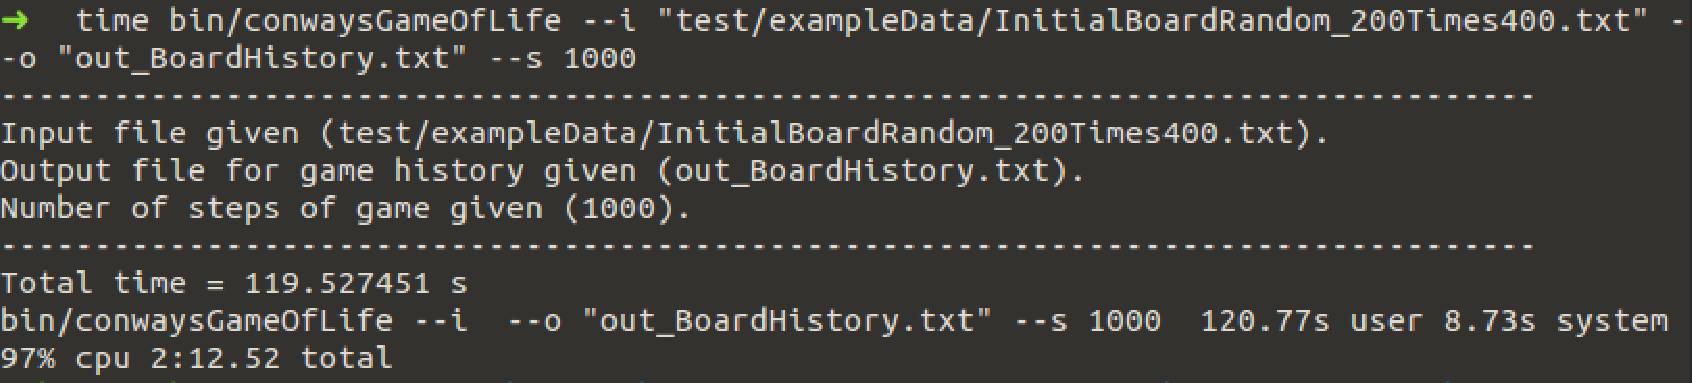
\includegraphics[width=0.95\textwidth]{figures/CommandLine_Serial.pdf}} \\
	\subfloat[Parallel implementation run]{\label{fig:resultsOMP}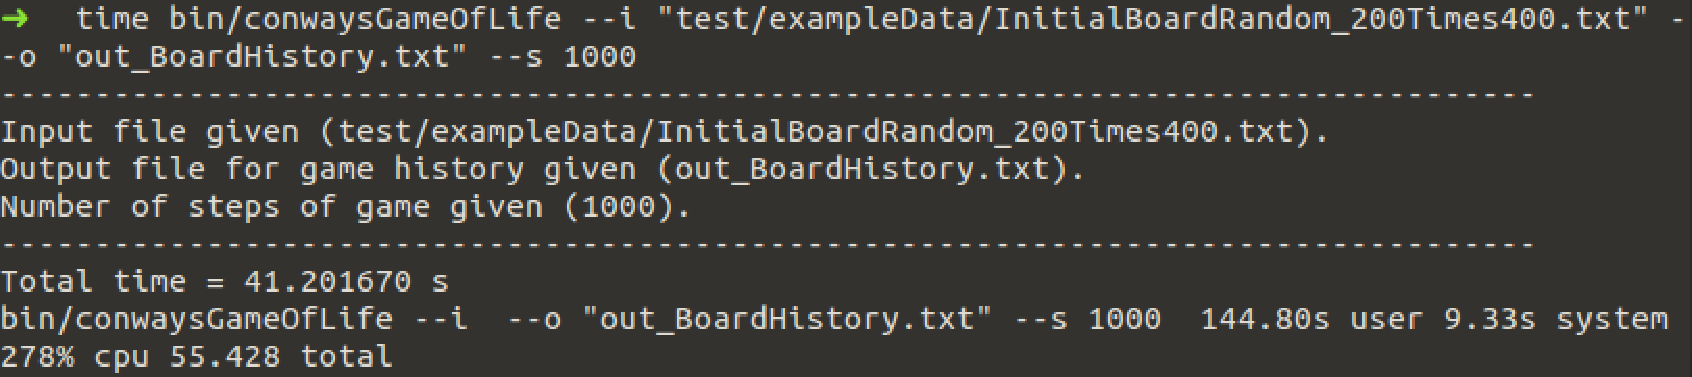
\includegraphics[width=0.95\textwidth]{figures/CommandLine_OpenMP.pdf}} 
	\caption{Statistic obtained via command 'time'}
	\label{fig:CommandLineResults}
\end{figure}

\smallskip

The respective cumulative computational times over the number of cells are illustrated in \cref{fig:computationalTimeOverCells} which states the expected roughly linear increase for each computational method. It can be observed that the implementation via OpenMP is already beneficial in lower numbers and becomes clearly evident in higher ones. However, the relative speed up seems to fluctuate.

\smallskip

In \cref{fig:computationalTimeOverIterations} the computational time is shown over iterations for selected boards. Again, the higher the number of cells the more severe the impact of OpenMP on cumulative time.

\smallskip

Lastly, \cref{fig:computationalTimeSpeedup} depicts the relative speed-up. In general, the advantage of using OpenMP becomes more apparent in higher number of cells. Since it was computed on 4 cores the theoretical maximum speed-up would be less than 4. However, the relative figures vary substantially over the number of cells. For a closer investigation larger boards could be investigated. Moreover, the fact that a virtual machine needed to be used could have had an impact on the results as well.

\begin{figure}\centering
	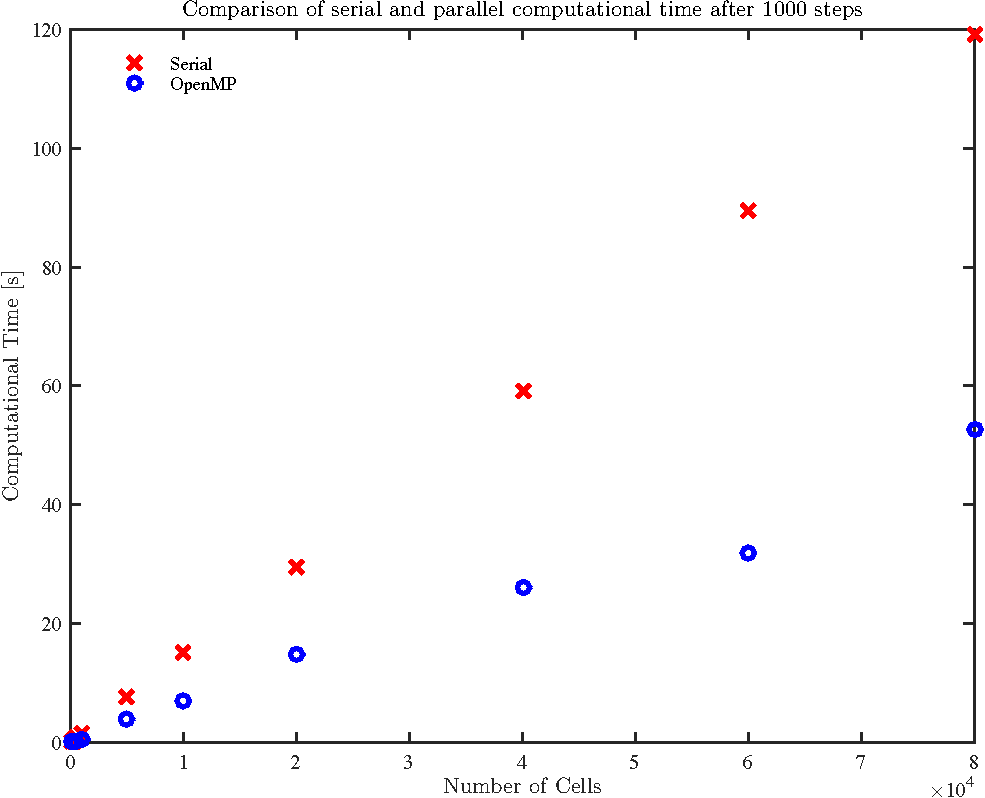
\includegraphics[width=0.8\textwidth]{figures/SerialOpenMP_Cells.pdf}
	\caption{Computational time over number of cells}
	\label{fig:computationalTimeOverCells}
\end{figure}

\begin{figure}\centering
	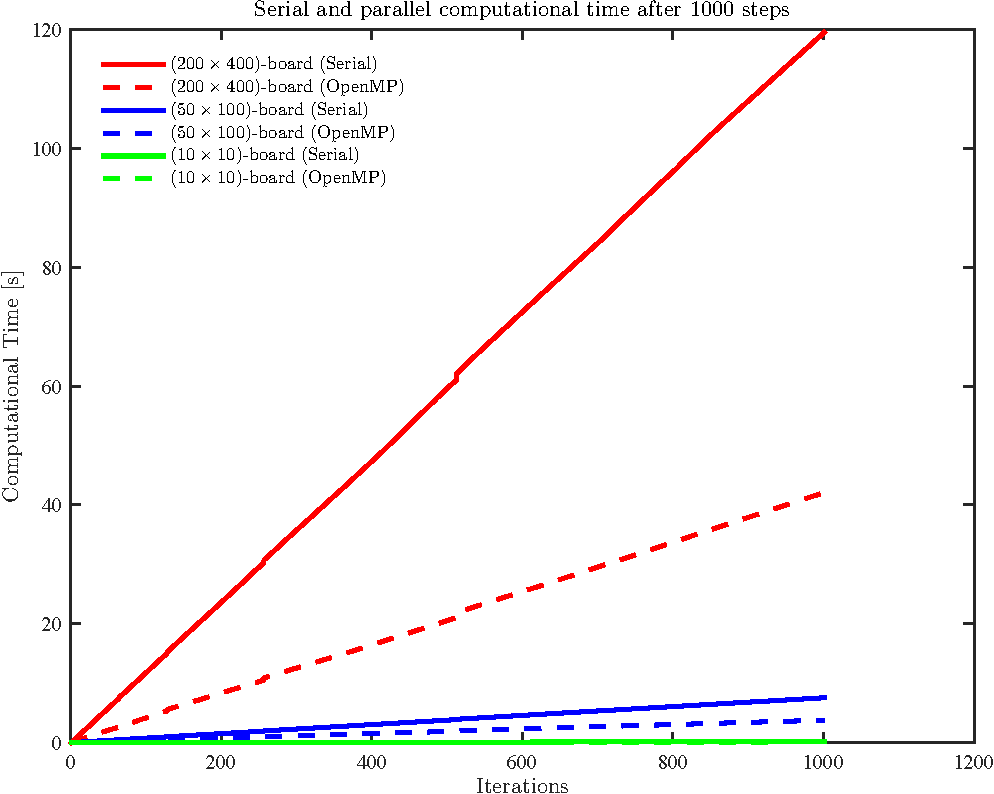
\includegraphics[width=0.8\textwidth]{figures/SerialOpenMP_Iterations.pdf}
	\caption{Computational time over number of iterations}
	\label{fig:computationalTimeOverIterations}
\end{figure}

\begin{figure}\centering
	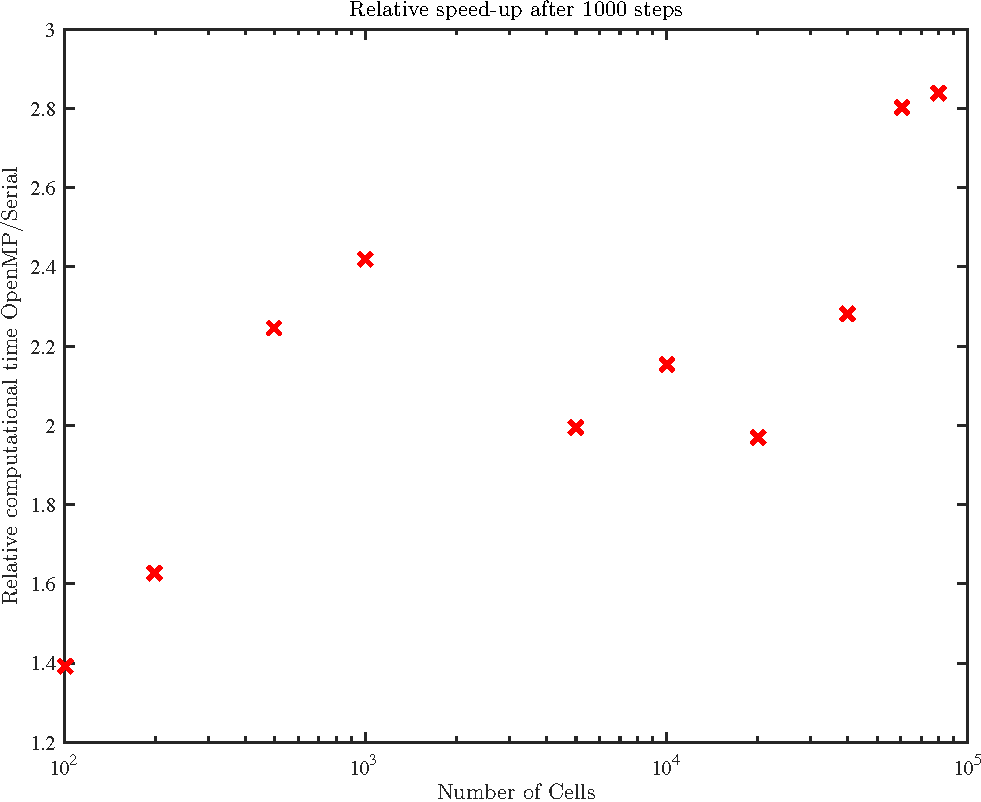
\includegraphics[width=0.8\textwidth]{figures/SerialOpenMP_Speedup.pdf}
	\caption{Relative speed-up}
	\label{fig:computationalTimeSpeedup}
\end{figure}

\cleardoublepage

%---Appendix*
%%%%%%%%%%%%%%%%%%%%%%%%%%%%%%%%%%%%%%%%%%%%%%%%%%%%%%%%%%%%%%%%%%%%%%%%%%%%%%%%%%%%%%%%%%%%%%%%%%%%%%%%%%%%%%%%%%%%%%%%
%\appendix
%\input{99_Appendix}

\cleardoublepage

%---Bibliography
%%%%%%%%%%%%%%%%%%%%%%%%%%%%%%%%%%%%%%%%%%%%%%%%%%%%%%%%%%%%%%%%%%%%%%%%%%%%%%%%%%%%%%%%%%%%%%%%%%%%%%%%%%%%%%%%%%%%%%%%
%\bibliographystyle{apalike} %other types: apalike, alpha, siam, abbrv, plain
%\bibliography{Bibliography.bib}
\end{document}
